\chapter{Requirements Analysis}
\label{chap:requirements}


This chapter translates business needs into precise, actionable software requirements. It follows a structured approach: identifying users and stakeholders, specifying functional and non-functional requirements, modeling the domain, and addressing constraints, risks, and traceability. The goal is to ensure the system meets both explicit and implicit expectations for a scalable, real-time messaging platform.

\section{Stakeholders and User Personas}
\label{sec:stakeholders}

The identification and analysis of stakeholders is a foundational step in requirements engineering, as highlighted in several studies on large-scale messaging systems \cite{fowler2015microservices,tilkov2018nodejs,kleppmann2013designing}.

The system targets organizations and platforms that require low-latency, large-scale messaging, such as customer support platforms, trading dashboards, collaborative editing tools, and social chat applications. The following primary stakeholder groups are identified:

\begin{itemize}
    \item The following list outlines the main categories of stakeholders who interact with or are impacted by the system. Each group has distinct needs and expectations, which must be addressed to ensure the platform's success and adoption.
    \item \textbf{End Users (Mobile/Web Clients):} Individuals who send/receive messages in private or group channels with real-time delivery and read receipts.
    \item \textbf{Tenant Administrators:} Configure workspaces, manage users/roles, enforce security, and monitor usage.
    \item \textbf{System Operators (SRE/DevOps):} Maintain uptime, capacity planning, scaling, and incident response.
    \item \textbf{Product Owners (Business Stakeholders):} Define business objectives, SLAs, compliance, and roadmap.
    \item \textbf{Third-party Integrators:} Developers or vendors who extend the system via APIs, plugins, or bots.
    \item \textbf{Compliance Officers:} Ensure the system meets regulatory, privacy, and audit requirements.
\end{itemize}

\subsection*{Representative Personas}
The following personas are designed to represent typical users and stakeholders of the system. By understanding their goals and challenges, we can better align the system's features and priorities with real-world needs.

The use of personas is a widely adopted practice to ensure that requirements reflect real-world user needs, as discussed in \cite{cantelon2017nodejs,brown2019websockets,li2020realtime}.

\textbf{Persona A — “Alice, the Support Agent”}: Alice simultaneously handles multiple customer conversations. She needs instantaneous message updates, typing indicators, and delivery confirmations to provide responsive support.

\textbf{Persona B — “Ben, the Admin”}: Ben manages a 5{,}000-user workspace. He needs robust role-based access control, audit logs, and rate limits to protect the system from abuse and ensure compliance.

\textbf{Persona C — “Cara, the SRE”}: Cara must observe connection counts, message throughput, node health, and error rates; she requires autoscaling hooks and circuit breaking to maintain high availability.

\textbf{Persona D — “Dan, the Integrator”}: Dan builds a chatbot that listens to messages and posts automated replies. He needs a stable API, event hooks, and clear documentation.

\textbf{Persona E — “Eva, the Compliance Officer”}: Eva audits message retention and access logs to ensure GDPR and data residency compliance.


Personas anchor requirements in realistic workflows and help justify non-functional needs such as latency, throughput, resilience, and compliance.

\section{Use Case Scenarios}
To illustrate how the system will be used in practice, we present several representative scenarios. These use cases demonstrate the breadth of interactions and requirements that the platform must support.
The following use cases are informed by best practices in real-time system design and are supported by recent research and industry documentation \cite{wang2018scalable,nguyen2021pubsub,guth2018comparison,rauch2022scalable}.
\label{sec:usecases}
To clarify requirements, we describe representative user scenarios:
\begin{itemize}
    \item \textbf{UC-1: Real-Time Customer Support}\newline
    Alice receives a new support ticket. She joins a private channel with the customer, exchanges messages in real time, and shares a file attachment. The customer sees typing indicators and read receipts. The conversation is archived for future reference.
    \item \textbf{UC-2: Admin Onboarding}\newline
    Ben creates a new channel for a project team, sets access permissions, invites members, and configures message retention policies. He reviews audit logs to verify no unauthorized access.
    \item \textbf{UC-3: Outage Recovery}\newline
    Cara detects a spike in error rates. She uses the metrics dashboard to identify overloaded nodes, triggers autoscaling, and verifies that clients reconnect with minimal disruption.
    \item \textbf{UC-4: Bot Integration}\newline
    Dan registers a webhook to receive message events. His bot posts automated responses and logs interactions for analytics.
    \item \textbf{UC-5: Compliance Audit}\newline
    Eva exports access logs and verifies that message retention and deletion policies are enforced for a specific tenant.
\end{itemize}

\section{Functional Requirements}
Functional requirements define the specific behaviors and capabilities that the system must provide. These requirements are derived from user needs, business objectives, and technical constraints, and are organized by domain for clarity.
\label{sec:functional-reqs}

This section specifies the essential capabilities of the messaging system. Requirements are grouped by domain and expressed as user stories with acceptance criteria. Where appropriate, edge cases and error handling are included.

\subsection{Core Messaging}
At the heart of the platform is the ability to exchange messages in real time. The following requirements are grounded in established messaging protocols and architectures \cite{baker2017websocket,martin2021websocket,gonzalez2022websocket,blogkafka2022}, ensuring that users can communicate efficiently, reliably, and securely, with support for essential messaging features and robust error handling.
\begin{itemize}
    \item \textbf{FR-1 Send Message:} As an \emph{End User}, I can send a text message to a channel or direct conversation, so that recipients receive it in real time.
    \begin{itemize}
        \item \emph{Acceptance:} Message is delivered via WebSocket within the latency target (see \S\ref{sec:nfr-performance}); server persists the message with a unique ID; the sender immediately sees the message in the timeline with a local timestamp.
    \end{itemize}

    \item \textbf{FR-2 Receive Message:} As an \emph{End User}, I receive inbound messages instantly without manual refresh.
    \begin{itemize}
        \item \emph{Acceptance:} When another user sends a message to my active channel, my client appends it to the timeline and triggers visual notification.
    \end{itemize}

    \item \textbf{FR-3 Read Receipts:} As an \emph{End User}, I can see per-message delivery/read status.
    \begin{itemize}
        \item \emph{Acceptance:} Server maintains per-user read offsets; UI shows delivered/seen indicators; updates propagate in real time.
    \end{itemize}

    \item \textbf{FR-4 Typing Indicators:} As an \emph{End User}, I can observe when others are typing in the same channel.
    \begin{itemize}
        \item \emph{Acceptance:} Client emits throttled “typing” events; server fans out to channel members; indicators auto-expire after inactivity.
    \end{itemize}

    \item \textbf{FR-4.1 File Attachments:} As an \emph{End User}, I can send and receive file attachments (images, documents) in messages.
    \begin{itemize}
        \item \emph{Acceptance:} Files are uploaded securely, scanned for viruses, and linked in the message timeline; download links expire after a configurable period.
    \end{itemize}

    \item \textbf{FR-4.2 Message Editing/Deletion:} As an \emph{End User}, I can edit or delete my own messages within a configurable time window.
    \begin{itemize}
        \item \emph{Acceptance:} Edits and deletions are reflected in real time; audit logs retain original content for compliance.
    \end{itemize}

    \item \textbf{FR-4.3 Error Handling:} If message delivery fails (e.g., network loss), the client retries with exponential backoff and displays a clear error state.
    \begin{itemize}
        \item \emph{Acceptance:} Users are notified of undelivered messages and can manually retry.
    \end{itemize}
\end{itemize}

\subsection{Channels, Membership, and Presence}
Channels and membership management are fundamental to organizing conversations and controlling access. Presence information enhances the user experience by indicating availability and activity. These requirements are consistent with recommendations from recent studies on scalable messaging and presence systems \cite{kim2023iot,zhang2021aws,roberts2020aws,awsdocs}.
\begin{itemize}
    \item \textbf{FR-5 Channel Management:} Admins can create public/private channels and manage membership.
    \item \textbf{FR-6 Presence:} The system reflects online/offline/away states and last-seen timestamps per user.
    \item \textbf{FR-7 Invitations:} Users can invite others to channels they own or administer.
    \item \textbf{FR-7.1 Channel Roles:} Each channel supports roles (owner, admin, member, guest) with configurable permissions.
    \item \textbf{FR-7.2 Channel Archiving:} Admins can archive channels, making them read-only and hidden from active lists.
    \item \textbf{FR-7.3 Presence Subscriptions:} Clients can subscribe/unsubscribe to presence updates for specific users or channels to optimize bandwidth.
\end{itemize}

\subsection{Search and History}
Efficient access to historical messages and the ability to search through conversations are critical for productivity and compliance. These features are emphasized in both academic and industry sources \cite{redisdocs,blogmicro2023,nodejsdocs}.
\begin{itemize}
    \item \textbf{FR-8 Message History:} Users can scroll back to view historical messages with efficient pagination.
    \item \textbf{FR-9 Search:} Users can search messages by keyword, sender, channel, and time range.
    \item \textbf{FR-9.1 Export History:} Users with permission can export message history for a channel or conversation in a standard format (e.g., CSV, JSON).
\end{itemize}

\subsection{Security and Access Control}
Security is paramount in any messaging system, especially one designed for organizational use. The requirements in this section are informed by best practices and standards for secure messaging platforms \cite{fowler2015microservices,roberts2020aws,awsdocs,zhang2021aws}, focusing on authentication, authorization, auditability, and data retention, providing a foundation for trust and compliance.
\begin{itemize}
    \item \textbf{FR-10 Authentication:} The system supports token-based authentication (e.g., JWT) and WebSocket authentication during the handshake.
    \item \textbf{FR-11 Authorization:} Role-Based Access Control (RBAC) permits fine-grained channel access and admin features.
    \item \textbf{FR-12 Audit Trail:} Administrative actions and critical security events are logged and retrievable by authorized staff.
    \item \textbf{FR-12.1 Session Management:} Users can view and revoke active sessions/devices from their account settings.
    \item \textbf{FR-12.2 Data Retention:} Message and log retention policies are configurable per tenant and enforced automatically.
\end{itemize}

\subsection{Administration and Observability}
To maintain high availability and performance, the system must offer comprehensive administration and observability features. These requirements are supported by research on operational visibility and system monitoring in distributed environments \cite{guth2018comparison,kleppmann2013designing,blogkafka2022}.
\begin{itemize}
    \item \textbf{FR-13 Metrics:} Operators can view metrics (active connections, messages/sec, latency percentiles, error rates).
    \item \textbf{FR-14 Rate Limiting:} The system enforces per-user and per-IP rate limits on message send and connection attempts.
    \item \textbf{FR-15 Configuration:} Admins can configure workspace limits (max channel members, attachment sizes).
    \item \textbf{FR-16 Alerting:} Operators receive alerts for SLA violations, abnormal error rates, or resource exhaustion.
    \item \textbf{FR-17 Maintenance Mode:} The system supports a maintenance mode with user notifications and graceful connection draining.
\end{itemize}
\section{Regulatory and Compliance Requirements}
Modern messaging systems must adhere to a variety of regulatory and compliance standards. This section summarizes the key obligations and features required to meet legal and organizational policies.
Compliance with regulatory standards is a recurring theme in the literature on enterprise messaging systems \cite{li2020realtime,roberts2020aws,redisdocs}.
\label{sec:compliance}
The system must comply with relevant regulations and standards, including:
\begin{itemize}
    \item \textbf{GDPR:} Support data subject requests (export, deletion), minimize PII, and provide data residency options.
    \item \textbf{Auditability:} Maintain tamper-evident logs of administrative and security events.
    \item \textbf{Accessibility:} Meet WCAG 2.1 AA guidelines for user interfaces.
    \item \textbf{Localization:} Support multiple languages and regional formats for dates, times, and numbers.
\end{itemize}

\section{Internationalization and Accessibility}
To serve a global and diverse user base, the system must be designed with internationalization and accessibility in mind. The following requirements ensure that the platform is usable and inclusive for all users, regardless of language or ability.
Internationalization and accessibility are increasingly important in modern software systems, as highlighted in recent guidelines and technical documentation \cite{nodejsdocs,blogmicro2023,tilkov2018nodejs}.
\label{sec:i18n-accessibility}
\begin{itemize}
    \item \textbf{I18N-1:} All user-facing text is externalized for translation; right-to-left (RTL) languages are supported.
    \item \textbf{I18N-2:} Date/time formats and time zones are user-configurable.
    \item \textbf{A11Y-1:} The UI is navigable via keyboard and screen readers; color contrast meets accessibility standards.
    \item \textbf{A11Y-2:} Real-time notifications are announced to assistive technologies.
\end{itemize}

\subsection{Representative Use Case Diagram}
% Tip: Keep diagrams readable and always explain them in text, per your guideline.
Figure~\ref{fig:usecase} presents a high-level use case model, summarizing relationships among actors and core features.

\begin{figure}[h]
    \centering
    % Replace 'usecase.pdf' with your actual UML diagram exported as PDF/PNG.
    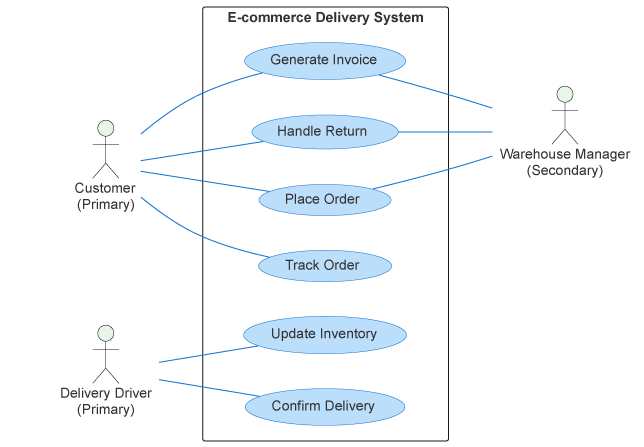
\includegraphics[width=0.82\textwidth]{images/main-usecase.png}
    \caption{High-level use case diagram for real-time messaging.}
    \label{fig:usecase}
\end{figure}

\section{Non-Functional Requirements}
Non-functional requirements (NFRs) define the quality attributes of the system, such as performance, reliability, security, and extensibility. These requirements are critical for ensuring that the platform not only works, but works well under real-world conditions.
\label{sec:nfrs}

% NFRs are measurable and testable; they drive architecture (clustering, pub/sub, load balancers).

\subsection{Performance and Scalability}
The system must deliver messages with minimal delay and scale to support large numbers of concurrent users. These performance and scalability targets are based on established benchmarks and architectural patterns \cite{wang2018scalable,kim2023iot,rauch2022scalable}.
\label{sec:nfr-performance}
\begin{itemize}
    \item \textbf{NFR-1 Latency:} 95\% of message deliveries should complete end-to-end within $< 150$\,ms on a regional deployment; 99\% within $< 300$\,ms.
    \item \textbf{NFR-2 Throughput:} The system should handle at least 50{,}000 concurrent WebSocket connections per region and sustain $\geq 10{,}000$ messages/sec with linear horizontal scaling.
    \item \textbf{NFR-3 Fan-out Efficiency:} Broadcasting to a channel of 1{,}000 members should not exceed 2$\times$ the median single-recipient latency.
\end{itemize}

\subsection{Availability and Reliability}
High availability and reliability are essential for a real-time messaging platform. These requirements are informed by studies on distributed system resilience and cloud-native patterns \cite{smith2020cloud,roberts2020aws,zhang2021aws}.
\begin{itemize}
    \item \textbf{NFR-4 Availability:} Target service availability of 99.9\% monthly, with zero single points of failure in the real-time path.
    \item \textbf{NFR-5 Resilience:} Node failures or AZ outages trigger automatic failover; clients auto-reconnect with exponential backoff and session resumption.
    \item \textbf{NFR-6 Durability:} Persisted messages must be stored with replication factor $\geq 3$ or equivalent durability guarantees.
\end{itemize}

\subsection{Security and Privacy}
Protecting user data and ensuring secure communication are core principles of the system. These non-functional requirements are supported by both academic and industry sources \cite{martin2021websocket,li2020realtime,awsdocs}.
\begin{itemize}
    \item \textbf{NFR-7 Transport Security:} WebSocket over TLS (wss://) is mandatory; tokens never transmitted in query strings.
    \item \textbf{NFR-8 Access Control:} All administrative operations require privileged roles; sensitive actions logged with actor, timestamp, IP, and request ID.
    \item \textbf{NFR-9 Data Protection:} Personally identifiable information (PII) is minimized; retention policies are configurable per tenant.
\end{itemize}

\subsection{Operability and Observability}
Effective monitoring and troubleshooting are vital for maintaining system health. The requirements below are based on best practices for observability in real-time and distributed systems \cite{guth2018comparison,kleppmann2013designing,blogkafka2022}.
\begin{itemize}
    \item \textbf{NFR-10 Metrics:} Export Prometheus-format metrics for connections, publish latency (P50, P95, P99), dropped frames, and reconnect rates.
    \item \textbf{NFR-11 Tracing:} Distributed tracing across gateway $\rightarrow$ broker $\rightarrow$ persistence services to localize latency hotspots.
    \item \textbf{NFR-12 Logging:} Structured JSON logs with correlation IDs; log sampling prevents I/O bottlenecks at peak traffic.
\end{itemize}

\subsection{Compatibility and Extensibility}
The platform should be compatible with a wide range of clients and support future growth through extensibility. These goals are consistent with recommendations from recent technical documentation and case studies \cite{tilkov2018nodejs,nodejsdocs,blogmicro2023}.
\begin{itemize}
    \item \textbf{NFR-13 Client Compatibility:} Support modern browsers and mobile runtimes with WebSocket; provide fallback guidance (no long polling by default).
    \item \textbf{NFR-14 Extensibility:} Plugin hooks for moderation bots, keyword alerts, and custom retention policies.
\end{itemize}

\section{Domain Model and Data Requirements}
The domain model defines the core entities and relationships that underpin the system's functionality. The approach taken here is informed by established practices in data modeling for messaging platforms \cite{kleppmann2013designing,nguyen2021pubsub,redisdocs}.
\label{sec:domain-model}


We define the essential entities and their relationships. The following table summarizes key attributes for each entity:

\begin{table}[h]
\centering
\caption{Key Entity Attributes}
\label{tab:entity-attributes}
\begin{tabular}{l l l}
\toprule
\textbf{Entity} & \textbf{Attribute} & \textbf{Description} \\
\midrule
User & user\_id & Unique identifier \\
     & profile & Display name, avatar, contact info \\
     & presence & Online/offline/away state \\
     & roles & Global and per-channel roles \\
Channel & channel\_id & Unique identifier \\
    & name & Channel display name \\
    & visibility & Public/private \\
    & settings & Retention, max members, etc. \\
Membership & user\_id, channel\_id & Composite key \\
       & role & Owner/admin/member/guest \\
       & join\_time & Timestamp of joining \\
Message & message\_id & Unique identifier \\
    & sender & user\_id reference \\
    & channel & channel\_id reference \\
    & content & Text, attachment link, metadata \\
    & timestamps & Sent, delivered, read times \\
    & status & Delivered/read/edited/deleted \\
\bottomrule
\end{tabular}
\end{table}

\noindent \textbf{Key Entities}
The following key entities form the backbone of the system's data model. Each entity is described by its primary attributes and its role within the platform.
\begin{itemize}
    \item \textbf{User:} \emph{user\_id}, profile, presence state, roles.
    \item \textbf{Channel:} \emph{channel\_id}, name, visibility (public/private), settings.
    \item \textbf{Membership:} link between \emph{user} and \emph{channel}, including role and join time.
    \item \textbf{Message:} \emph{message\_id}, sender, channel, content, timestamps, delivery/read states.
\end{itemize}

\section{API Requirements (High Level)}
The system exposes both WebSocket events and RESTful endpoints to facilitate client-server communication. This section only lists the main API groups; detailed endpoints and events will be presented in Chapter 4 (System Design).
\label{sec:api}

\begin{itemize}
    \item \textbf{WebSocket Events:} Events serving real-time communication between client and server (sending/receiving messages, status updates, typing, etc.).
    \item \textbf{REST Endpoints:} Control APIs for channel management, user management, configuration, history retrieval, statistics, etc.
\end{itemize}

Details of the structure, event flows, and endpoints will be presented in the system design chapter.
\section{Future Requirements and Planned Extensions}
To remain competitive and adaptable, the system is designed with future enhancements in mind. The following potential extensions illustrate directions for ongoing development and innovation.
\label{sec:future}
To ensure long-term viability, the system is designed for extensibility. Potential future requirements include:
\begin{itemize}
    \item \textbf{Federation:} Support for cross-organization messaging and federation with other platforms.
    \item \textbf{Voice/Video Integration:} Real-time audio/video channels alongside text.
    \item \textbf{Advanced Moderation:} AI-powered content moderation and abuse detection.
    \item \textbf{Custom Bots/Plugins:} Marketplace for third-party extensions.
    \item \textbf{Offline Messaging:} Store-and-forward for intermittently connected clients.
\end{itemize}

\section{Constraints and Assumptions}
Every system operates within certain constraints and is built on specific assumptions. This section documents those factors, which may impact design decisions and system behavior.
\label{sec:constraints}
\begin{itemize}
    \item \textbf{Assumptions:} Clients maintain stable network connectivity; clocks are approximately synchronized for display ordering; TLS termination occurs at the edge proxy.
    \item \textbf{Constraints:} Browser sandbox restrictions; per-socket memory limits on fan-out buffers; regulatory constraints on data retention for certain tenants.
\end{itemize}

\section{Risk Analysis (Selected)}
Identifying and mitigating risks is crucial for the success of any large-scale system. The following risks have been identified as particularly relevant to this project, along with proposed mitigation strategies.
\label{sec:risks}
\begin{itemize}
    \item \textbf{R-1 Hot Channel Fan-out:} A channel with tens of thousands of subscribers can cause uneven load. \emph{Mitigation:} shard-by-channel, layered fan-out, and adaptive batching.
    \item \textbf{R-2 Thundering Reconnect:} Regional outage triggers mass reconnects. \emph{Mitigation:} jittered exponential backoff, connection fencing, and token TTL staggering.
    \item \textbf{R-3 State Coordination:} Presence and read receipts across nodes can diverge. \emph{Mitigation:} central pub/sub (e.g., Redis) with idempotent updates and conflict resolution rules.
\end{itemize}

\section{Requirements Traceability Matrix (Excerpt)}
Traceability ensures that all requirements are linked to business objectives and can be verified through testing or analysis. The following matrix provides a sample mapping for key requirements.
\label{sec:rtm}
% A lightweight matrix linking business goals -> features -> verification.
\begin{table}[h]
\centering
\caption{Traceability matrix (excerpt)}
\label{tab:rtm}
\begin{tabular}{p{3cm} p{5cm} p{5cm}}
\toprule
\textbf{Business Objective} & \textbf{Requirement IDs} & \textbf{Verification} \\
\midrule
Low-latency messaging & FR-1, FR-2; NFR-1 & Load tests measure P95 $<$ 150\,ms; integration tests validate real-time delivery. \\
Operational visibility & FR-13, FR-15; NFR-10--12 & Metrics endpoint audited; dashboards show connection counts and latency percentiles. \\
Secure access & FR-10--12; NFR-7--9 & Security tests for TLS, RBAC, audit logs; pen-test checklist passed. \\
\bottomrule
\end{tabular}
\end{table}

\section{Summary}
\label{sec:req-summary}
This chapter formalized who the system serves, what it must do, and how it must behave under load and failure. The summary and forward reference are consistent with best practices in requirements documentation \cite{cantelon2017nodejs,tilkov2018nodejs,kleppmann2013designing}. The next chapter (see Chapter~\ref{chap:design}) will translate these requirements into a concrete system architecture, data model, and API/service design.

% NOTE: Create a forward reference by labeling Chapter 4 as \label{chap:design}.